% Options for packages loaded elsewhere
\PassOptionsToPackage{unicode}{hyperref}
\PassOptionsToPackage{hyphens}{url}
\PassOptionsToPackage{dvipsnames,svgnames,x11names}{xcolor}
%
\documentclass[
  12pt]{article}

\usepackage{amsmath,amssymb}
\usepackage{iftex}
\ifPDFTeX
  \usepackage[T1]{fontenc}
  \usepackage[utf8]{inputenc}
  \usepackage{textcomp} % provide euro and other symbols
\else % if luatex or xetex
  \usepackage{unicode-math}
  \defaultfontfeatures{Scale=MatchLowercase}
  \defaultfontfeatures[\rmfamily]{Ligatures=TeX,Scale=1}
\fi
\usepackage{lmodern}
\ifPDFTeX\else  
    % xetex/luatex font selection
\fi
% Use upquote if available, for straight quotes in verbatim environments
\IfFileExists{upquote.sty}{\usepackage{upquote}}{}
\IfFileExists{microtype.sty}{% use microtype if available
  \usepackage[]{microtype}
  \UseMicrotypeSet[protrusion]{basicmath} % disable protrusion for tt fonts
}{}
\makeatletter
\@ifundefined{KOMAClassName}{% if non-KOMA class
  \IfFileExists{parskip.sty}{%
    \usepackage{parskip}
  }{% else
    \setlength{\parindent}{0pt}
    \setlength{\parskip}{6pt plus 2pt minus 1pt}}
}{% if KOMA class
  \KOMAoptions{parskip=half}}
\makeatother
\usepackage{xcolor}
\usepackage[margin=0.8in]{geometry}
\setlength{\emergencystretch}{3em} % prevent overfull lines
\setcounter{secnumdepth}{-\maxdimen} % remove section numbering
% Make \paragraph and \subparagraph free-standing
\ifx\paragraph\undefined\else
  \let\oldparagraph\paragraph
  \renewcommand{\paragraph}[1]{\oldparagraph{#1}\mbox{}}
\fi
\ifx\subparagraph\undefined\else
  \let\oldsubparagraph\subparagraph
  \renewcommand{\subparagraph}[1]{\oldsubparagraph{#1}\mbox{}}
\fi


\providecommand{\tightlist}{%
  \setlength{\itemsep}{0pt}\setlength{\parskip}{0pt}}\usepackage{longtable,booktabs,array}
\usepackage{calc} % for calculating minipage widths
% Correct order of tables after \paragraph or \subparagraph
\usepackage{etoolbox}
\makeatletter
\patchcmd\longtable{\par}{\if@noskipsec\mbox{}\fi\par}{}{}
\makeatother
% Allow footnotes in longtable head/foot
\IfFileExists{footnotehyper.sty}{\usepackage{footnotehyper}}{\usepackage{footnote}}
\makesavenoteenv{longtable}
\usepackage{graphicx}
\makeatletter
\def\maxwidth{\ifdim\Gin@nat@width>\linewidth\linewidth\else\Gin@nat@width\fi}
\def\maxheight{\ifdim\Gin@nat@height>\textheight\textheight\else\Gin@nat@height\fi}
\makeatother
% Scale images if necessary, so that they will not overflow the page
% margins by default, and it is still possible to overwrite the defaults
% using explicit options in \includegraphics[width, height, ...]{}
\setkeys{Gin}{width=\maxwidth,height=\maxheight,keepaspectratio}
% Set default figure placement to htbp
\makeatletter
\def\fps@figure{htbp}
\makeatother

\usepackage{datetime}
\newdateformat{mydate}{\monthname[\THEMONTH], \THEYEAR}
\usepackage{fancyhdr}
\fancyhf{}
\pagestyle{fancy}
\lhead{\mydate{\today}}
\rhead{Reuse: \href{https://creativecommons.org/licenses/by-nc-sa/3.0/}{CC BY-NC-SA 3.0}}
\makeatletter
\@ifpackageloaded{caption}{}{\usepackage{caption}}
\AtBeginDocument{%
\ifdefined\contentsname
  \renewcommand*\contentsname{Table of contents}
\else
  \newcommand\contentsname{Table of contents}
\fi
\ifdefined\listfigurename
  \renewcommand*\listfigurename{List of Figures}
\else
  \newcommand\listfigurename{List of Figures}
\fi
\ifdefined\listtablename
  \renewcommand*\listtablename{List of Tables}
\else
  \newcommand\listtablename{List of Tables}
\fi
\ifdefined\figurename
  \renewcommand*\figurename{Figure}
\else
  \newcommand\figurename{Figure}
\fi
\ifdefined\tablename
  \renewcommand*\tablename{Table}
\else
  \newcommand\tablename{Table}
\fi
}
\@ifpackageloaded{float}{}{\usepackage{float}}
\floatstyle{ruled}
\@ifundefined{c@chapter}{\newfloat{codelisting}{h}{lop}}{\newfloat{codelisting}{h}{lop}[chapter]}
\floatname{codelisting}{Listing}
\newcommand*\listoflistings{\listof{codelisting}{List of Listings}}
\makeatother
\makeatletter
\makeatother
\makeatletter
\@ifpackageloaded{caption}{}{\usepackage{caption}}
\@ifpackageloaded{subcaption}{}{\usepackage{subcaption}}
\makeatother
\ifLuaTeX
  \usepackage{selnolig}  % disable illegal ligatures
\fi
\usepackage{bookmark}

\IfFileExists{xurl.sty}{\usepackage{xurl}}{} % add URL line breaks if available
\urlstyle{same} % disable monospaced font for URLs
\hypersetup{
  pdftitle={Reference Solutions for MA121 Final Review},
  pdfauthor={Dr.~Ye},
  colorlinks=true,
  linkcolor={blue},
  filecolor={Maroon},
  citecolor={Blue},
  urlcolor={Blue},
  pdfcreator={LaTeX via pandoc}}

\title{Reference Solutions for MA121 Final Review}
\author{Dr.~Ye}
\date{June, 2024}

\begin{document}
\maketitle
\begin{abstract}
Those references solutions are for QCC MA121 final review (Version
Summer 2024). A html version can be found at
\url{https://fyeteaching.github.io/RefSolMA121/index.html}. Please let
me know if you see any mistakes. Thank you!
\end{abstract}

\begin{enumerate}
\def\labelenumi{\arabic{enumi}.}
\item
  To convert an angle from radians to degree, multiply the angle by
  \(\frac{180^\circ}{\pi}\). So
  \[\frac{5\pi}{6}\cdot\frac{180^\circ}{\pi}=150^\circ.\]
\item
  Using the definition of cosine, the length of \(AC\) satsifies the
  equation \(\cos 40^\circ=\frac{AC}{200 \text{ m}}\). So
  \[AC=200 \text{ m} \cdot \cos 40^\circ \approx 153.2 \text{ m}.\]
\item
  To get a cofunction with same value, replace the given angle by its
  complement. So
  \[\csc\left(\dfrac{2\pi}{5}\right)=\sec\left(\frac{\pi}{2}-\frac{2\pi}{5}\right)=\sec\sec\left(\frac{5\pi}{10}-\frac{4\pi}{10}\right)=\sec\left(\frac{\pi}{10}\right).\]
\item
  Let \(A\) be the end of the ramp on the street, \(B\) the end of the
  ramp at the entrance of the clinic, \(C\) is the point on the street
  right below \(B\).

  \begin{figure}[H]

  {\centering 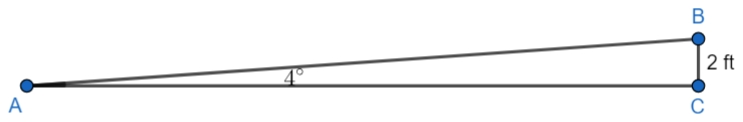
\includegraphics{Q4.jpeg}

  }

  \caption{Right triangle with an angle 4 degrees and opposite side 2}

  \end{figure}%

  The length of the ramp \(AB\) is the hypotenuse of the right triangle
  \(\triangle ABC\). The length of the street \(AC\) is the adjacent
  side of the right triangle and the height of the building \(BC\) is
  the opposite side of the right triangle. The angle of elevation is the
  angle between the street and the ramp, that is, \(\angle A\). With
  \(\angle A = 4^\circ\), \(BC =  2 \text{ ft}\), the length of the ramp
  satisfies the equation \(\tan 4^\circ = \frac{2 \text{ ft}}{AC}\).
  Solving for \(AC\) gives the length of the ramp
  \[AC = \frac{2 \text{ ft}}{\tan 4^\circ} \approx 28.6 \text{ ft}.\]
\item
  The reference angle is the acute angle formed by the terminal side and
  the \(x\)-axis. Once the terminal side is determined, the reference
  angle can be found by measuring the angle between the terminal side
  and the \(x\)-axis. The angle of \(242^\circ\) has the terminal side
  in the third quadrant. The reference angle is
  \(242^\circ-180^\circ=62^\circ\).
\item
  To convert an angle from radian to degree, multiply the angle by
  \(\frac{180^\circ}{\pi}\). So
  \[135^\circ = \frac{135\pi}{180} = \frac{3\pi}{4}.\]
\item
  From the definition of sine and cosine of an arbitrary angle
  \(\theta\), \(x = r\cos\theta\) and \(y = r\sin\theta\), where
  \((x, y)\) is a point on the terminal side and \(r\) is the distance
  from the origin. Because \(\csc\theta = 1/\sin\theta <0\) and
  \(\sec\theta = 1/\cos\theta >0\), then a point on the terminal side
  has \(y<0\) and \(x>0\). So the terminal side is in the fourth
  quadrant.
\item
  The find \(\sin \theta\) from a given point on the terminal side,
  divide the \(y\)-coordinate by the distance from the origin. In this
  case, the distance between \((-3, 4)\) and the origin is
  \(\sqrt{x^2+y^2}=\sqrt{(-3)^2+4^2} = 5\). So
  \[\sin \theta = \frac{y}{r} = \frac{-3}{5}.\]
\item
  Coterminal angles are different angles that have the same terminal
  side. To find a coterminal angle, add or subtract a multiple of
  \(360^\circ\) (or \(2\pi\)) to the given angle. Since the given angle
  is negative and desired coterminal angle is positive and less than
  \(360^\circ\). We add multiples of \(360^\circ\) so that the angle is
  positive and less than \(360^\circ\). So the desired coterminal angle
  is \[-685^\circ + 2\cdot 360^\circ = 35^\circ.\]
\item
  To determine the exact value of \(\sin\theta\) with the given measure
  of \(\theta\), one can use the reference angle
  \(\theta_{\text{ref}}\). If the terminal side is in Quadrant I or II
  (\(y>0\)), then \(\sin\theta =\sin \theta_{\text{ref}}\). Otherwise,
  \(\sin\theta = -\sin \theta_{\text{ref}}\). In this case, the terminal
  side of \(\dfrac{4\pi}{3}\) is in Quadrant III, and the reference
  angle is \(\dfrac{\pi}{3}\). Therefore,
  \[\sin \dfrac{4\pi}{3} = -\sin \dfrac{\pi}{3} = -\frac{\sqrt{3}}{2}.\]
  \textbf{Remark:} Trig of special angles in \([0, \frac{\pi}{2}]\) can
  be found using the left hand trick. See for example
  \url{https://www.geogebra.org/m/cGKXJnxZ}.
\item
  For a function \(y= A\cos(Bx)\), the amplitude is \(|A|\) and the
  period is \(\dfrac{2\pi}{|B|}\). In this case, the amplitude is
  \(|3|=3\) and the period is \(\dfrac{2\pi}{|\frac{\pi}{6}|}=12\). To
  sketch the graph within one period, first find the 5 key points: the
  maximum, the minimum, the points on the middle. When inside function
  is simple \(Bx\), the first point can be taken as
  \((0, A\cos(0))=(0, -3)\). Let \(T\) be the period. The second point
  can be taken as
  \(\left(\dfrac{T}{4}, A\cos(\dfrac{\pi}{2})\right)=(3, 0)\), the third
  point can be taken as
  \(\left(\dfrac{T}{2}, A\cos(\pi)\right)=(6, 3)\), the fourth point can
  be taken as
  \(\left(\dfrac{3T}{4}, A\cos(\dfrac{3\pi}{2})\right)=(9, 0)\), and the
  fifth point can be taken as \(\left(T, A\cos(2\pi)\right)=(12, -3)\).
  Then connect the points smoothly to get the graph.

  \begin{figure}[H]

  {\centering 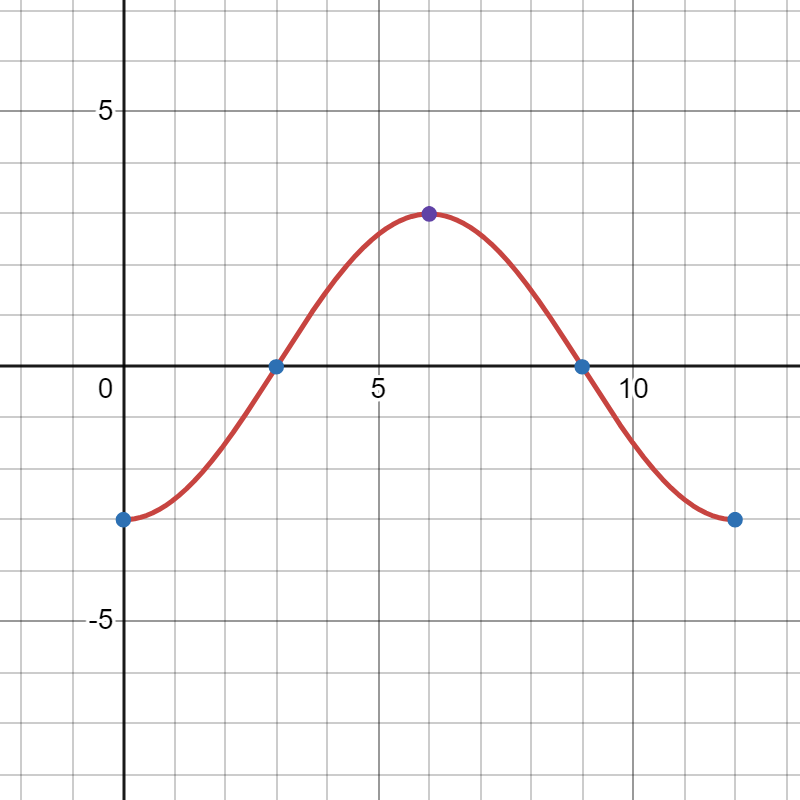
\includegraphics[width=0.6\textwidth,height=\textheight]{Q11.png}

  }

  \caption{Graph of y=-3cos(pi/6*x)}

  \end{figure}%
\item
  The reference angle is the acute angle formed by the terminal side and
  the \(x\)-axis. Once the terminal side is determined, the reference
  angle can be found by measuring the angle between the terminal side
  and the \(x\)-axis. The angle of \(\dfrac{8\pi}{9}\) has the terminal
  side in the second quadrant. The reference angle is
  \[ \pi-\frac{8\pi}{9}=\frac{\pi}{9}. \]
\item
  Given \(\sin\beta\), the value of \(\cos\theta\) can be find
  algebraically using the Pythagorean identity
  \(\sin^2\theta + \cos^2\theta = 1\). Since \(\sin\beta = \dfrac89\)
  and \(beta\) is acute,
  \(\cos\beta = \sqrt{1-\sin^2\beta} = \sqrt{1-\left(\dfrac89\right)^2} = \dfrac{\sqrt{17}}{9}\).

  The value of \(\cos\beta\) can be found using the right triangle. Let
  \(\angle C\) be the right angle and \(A\) be the given angle. Take the
  hypotnuse \(AB=9\) and the opposite side \(BC=8\). Then by the
  geometric Pythogorean theorem, \(AC=\sqrt{9^2-8^2}= \sqrt{17}\). So
  \(\cos\beta = \dfrac{AC}{AB} = \dfrac{\sqrt{17}}{9}\).
\item
  Since the angle of \(120^\circ\) is in the second quadrant, the
  reference angle is \(180^\circ-120^\circ=60^\circ\). The value of
  \(\tan 120^\circ\) can be found using the reference angle. Since
  \(\tan 60^\circ = \sqrt{3}\), then
  \(\tan 120^\circ = -\tan 60^\circ = -\sqrt{3}\).
\item
  Because \(\tan\theta < 0\), the termial side of \(\theta\) is in the
  second or the fourth quadrant. Because \(\cos\theta < 0\), the
  terminal side of \(\theta\) is in the second quadrant.
\item
  Let \(A\) be the observation point on the ground, \(B\) be the top of
  the building, and \(C\) be the bottom of the building. Note that
  \(\angle C\) is the right angle, and \(\angle A =71^\circ\).

  \begin{figure}[H]

  {\centering 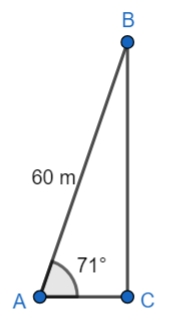
\includegraphics{Q16.jpeg}

  }

  \caption{Right triangle with hypotenuse 60 and an angle 71 degrees}

  \end{figure}%

  Because the distance between \(A\) and \(C\) is 60 meters. The hight
  of the building \(BC\) is the opposite side of the angle \(\angle A\).
  By the definition of sine,
  \(\sin 71^\circ = \dfrac{BC}{60 \text{ m}}\). Solving for \(BC\) gives
  the height of the building
  \[BC = 60 \text{ m} \cdot \sin 71^\circ \approx 174.3 \text{ m}.\]
\item
  Since \(\theta\) is acute and \(\cos\theta = \dfrac67\). Then
  \[\sin\theta=\sqrt{1-\left(\dfrac67\right)^2} = \dfrac{\sqrt{13}}{7}.\]
\item
  Since \(A\) is in the third quadrant, then \(\cos A\) is negative.
  Using the Pythagorean identity \(\sin^2A + \cos^2A = 1\), we have
  \(\cos A = -\sqrt{1-\sin^2A} = -\sqrt{1-\left(-\dfrac{\sqrt{3}}{4}\right)^2} = -\dfrac{\sqrt{13}}{4}\).
  Using the quotient identity \(\tan A = \dfrac{\sin A}{\cos A}\), we
  have
  \[\tan A = \dfrac{-\dfrac{\sqrt{3}}{4}}{-\dfrac{\sqrt{13}}{4}} = \dfrac{\sqrt{39}}{13}.\]
\item
  Similar to Question 11, the amplitude is \(|A|=|2|=2\), the period is
  \(\dfrac{2\pi}{|B|}=\dfrac{2\pi}{|\frac{1}{3}|}=6\pi\).

  The 5 key points are \((0, 0)\), \((1.5\pi, 2)\), \((2\pi, 0)\),
  \((4.5\pi, -2)\), and \((6\pi, 0)\). Connect the points smoothly to
  get the graph.

  \begin{figure}[H]

  {\centering 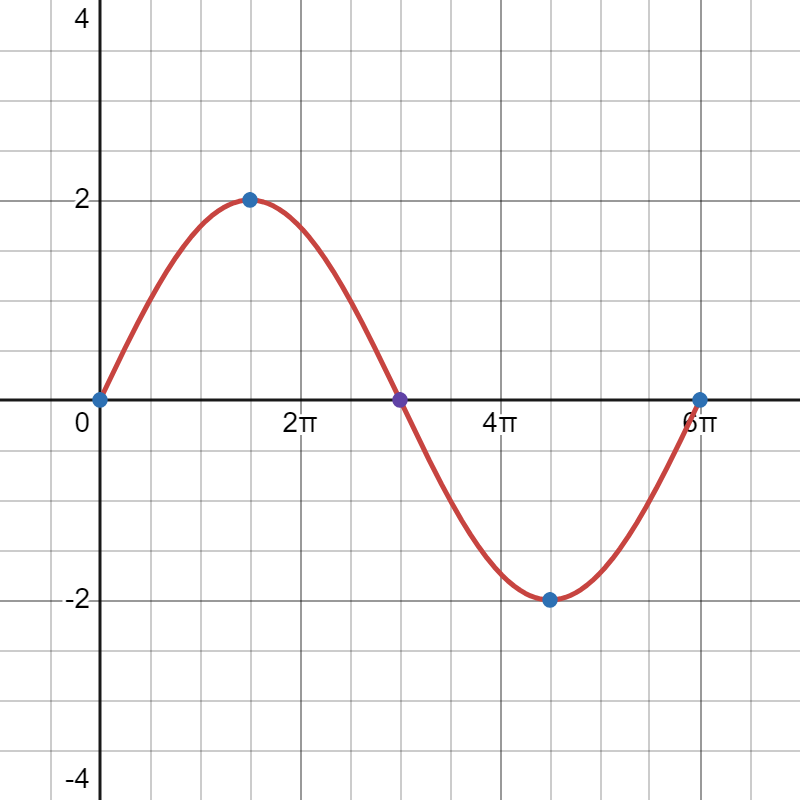
\includegraphics[width=0.6\textwidth,height=\textheight]{Q19.png}

  }

  \caption{Graph of y=2sin(x/3)}

  \end{figure}%
\item
  Since \(\tan\theta = -\frac12\) and \(\cos\theta>0\), the angle
  \(\theta\) is fourth quadrant. To find the values of the trigonometric
  functions without sign, we can apply the geometric method to
  \(\theta_{\text{ref}}\) as see in Question 13. Consider the triangle
  with the opposite side \(1\) and the adjacent side \(2\). The
  hypotenuse is \(\sqrt{1^2+2^2}=\sqrt{5}\). Then
  \(\sin\theta_{\text{ref}} = \dfrac{1}{\sqrt{5}}\),
  \(\cos\theta_\text{ref} = \dfrac{2}{\sqrt{5}}\). Therefore,
  \[\sin\theta = -\dfrac{\sqrt{5}}{5},\]
  \[\cos\theta = \dfrac{2\sqrt{5}}{5},\] \[\tan\theta = -\dfrac{1}{2},\]
  \[\csc\theta = -\sqrt{5},\] \[\sec\theta = \dfrac{\sqrt{5}}{2},\]
  \[\cot\theta = -2.\]
\item
  The cofunction with the same value as \(\tan 78^\circ\) is
  \(\cot(90^\circ-78^\circ)=\cot 12^\circ\).
\item
  Since the given angle is greater than \(2\pi\), to find the cotermimal
  angle in \([0, 2\pi]\), we subtract multiples of \(2\pi\) from the
  given angle. So the coterminal angle in \([0, 2\pi]\) is
  \[\dfrac{17\pi}{5} - 2\pi = \dfrac{7\pi}{5}.\]
\item
  Let \(A\) be the bottom of the ladder, \(B\) the top of the ladder,
  and \(C\) the point on the ground right below \(B\).

  \begin{figure}[H]

  {\centering 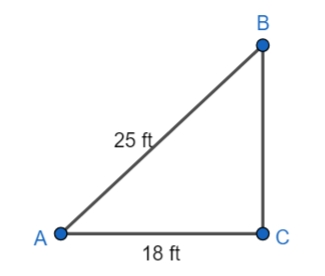
\includegraphics{Q23.jpeg}

  }

  \caption{Right triangle with hypotenuse 25 and adjacent 18}

  \end{figure}%

  Since the ladder is 25-foot long and the bottom of the ladder is 18
  feet from the wall, we have \(AC=18\) and \(AB=25\). The angle formed
  by the ladder and the ground is \(\angle A\), which statisfies the
  equation \(\cos A = \dfrac{18}{25}\). Solving for \(A\) gives the
  angle \[A = \cos^{-1}\left(\dfrac{18}{25}\right) \approx 44^\circ.\]

  The height of the top of the ladder can be calculated by
  \(BC = 25\sin A \approx 25\sin 44^\circ \approx 17.3\) feet.

  Note that \(BC\) can also be found using the Pythagorean theorem:
  \[BC = \sqrt{25^2-18^2} = \sqrt{625-324} = \sqrt{301} \approx 17.3 \text{ ft}.\]
\item
  Let \(A\) be the starting point of the road, \(B\) the ending point on
  the road, and \(C\) the point such that the triangle \(\triangle ABC\)
  is a right triangle with \(C\) the right angle.

  \begin{figure}[H]

  {\centering 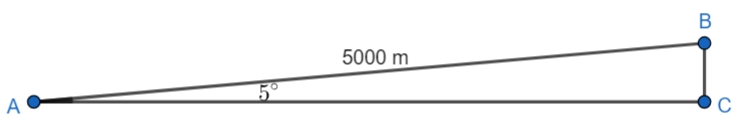
\includegraphics{Q24.jpeg}

  }

  \caption{Right triangle with hypotenuse 5000 and an angle 5 degrees}

  \end{figure}%

  Since the driving distance is 5000 meters and the angle of elevation
  is \(5^\circ\), the increase in altitude is the opposite side \(BC\)
  of the right triangle. By the definition of sine, we have
  \[\sin 5^\circ = \dfrac{BC}{5000 \text{ m}}.\] Solving for \(BC\)
  gives the increase in altitude
  \[BC = 5000 \text{ m} \cdot \sin 5^\circ \approx 436 \text{ m}.\]
\item
  To convert from radian to degree, multiply the angle by
  \(\dfrac{180^\circ}{\pi}\). So
  \[2 \cdot \dfrac{180^\circ}{\pi} \approx 114.59^\circ.\]
\item
  Since the point is on the unit circle, the distance from the origin is
  1. The value of \(\cos\theta\) is the \(x\)-coordinate of the point.
  So \(\cos\theta = \dfrac{1}{2}\). The value of \(\sin\theta\) is the
  \(y\)-coordinate of the point. Because the point is in the fourth
  quadrant, \(y\)-coordinate is negative. So by the Pythagorean
  identity,
  \[\sin\theta = -\sqrt{1-\cos^2\theta} = -\sqrt{1-\left(\dfrac{1}{2}\right)^2} = -\dfrac{\sqrt{3}}{2}.\]
\item
  The distance \(r\) from the point on the termimal side to the origin
  is
  \[r=\sqrt{x^2+y^2}=\sqrt{\left(-\frac{7}{25}\right)^2 + \left(\frac{24}{25}\right)^2}=1.\]
  Therofore, by the definition of trigonometric functions of an angle
  \(\theta\), we have \[\sin\theta = \frac{y}{r} = \frac{24}{25},\]
  \[\cos\theta = \frac{x}{r} = -\frac{7}{25},\]
  \[\tan\theta = \frac{y}{x} = -\frac{24}{7},\]
  \[\cot\theta = \frac{x}{y} = -\frac{7}{24}.\]
  \[\sec\theta = \frac{r}{x} = -\frac{25}{7},\]
  \[\csc\theta = \frac{r}{y} = \frac{25}{24},\]
\item
  Similar to Question, the distance \(r\) is
  \(r=\sqrt{12^2+(-5)^2}=13\). Hence the trigonometric functions are
  \[\sin A = \frac{y}{r} = -\frac{5}{13},\]
  \[\cos A = \frac{x}{r} = \frac{12}{13},\]
  \[\tan A = \frac{y}{x} = -\frac{5}{12},\]
  \[\cot A = \frac{x}{y} = -\frac{12}{5}.\]
  \[\sec A = \frac{r}{x} = \frac{13}{12},\]
  \[\csc A = \frac{r}{y} = -\frac{13}{5},\]
\end{enumerate}



\end{document}
